\chapter{HASIL DAN PEMBAHASAN}
\label{BAB4:hasil}

\section{\textit{Text Preprocessing}}

Data yang telah dikumpulkan berupa 333 dokumen dengan abstrak, pada penelitian ini akan dipakai sehingga berisi 333 baris. Setelah itu, dilakukan suatu \textit{text preprocessing} pada teks tersebut. Pada setelah langkah \textit{text preprocessing} teks tersebut, akan dibagi menjadi dua alur sebagaimana yang telah digambarkan pada Gambar \ref{fig:3-3}, yang pertama ialah sebelum dilakukan suatu pengelompokkan abstrak serupa menjadi klaster dan yang alur lainnya sebelum dilakukan pemilihan kata dasar untuk mencari kata kunci yang relevan dengan teori Luhn.

Adapun tahapan dalam \textit{text preprocessing} hingga mendapatkan hasil berupa kata kunci yang dicari digambarkan pada gambar di bawah ini:
\begin{figure}[H]
    \centering
    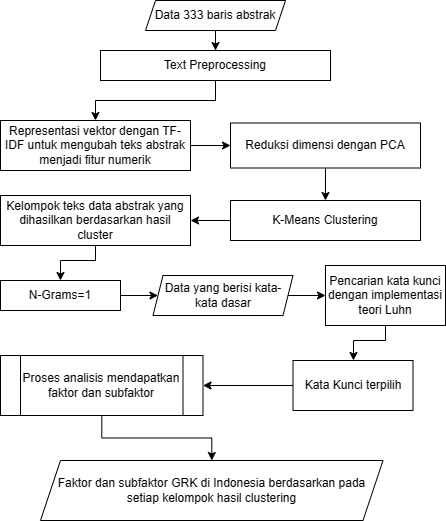
\includegraphics[width=0.75\linewidth]{img/bab4-1.png}
    \caption{Proses tahapan \textit{text preprocessing} hingga hasil menggunakan data studi literatur}
    \label{fig:4-1}
\end{figure}

Di bawah ini, merupakan teknik berupa istilah yang digunakan pada saat melakukan \textit{text preprocessing} sebagai berikut:
\begin{enumerate}
    \item \textit{Lowercase}: Membuat semua teks pada data tersebut menjadi bukan huruf kapital.
    \item \textit{Punctuation}: Menghapus semua unsur tanda baca.
    \item \textit{Stopword}: Menghapus unsur kata-kata yang tidak bermakna, seperti '\textit{is, a, it, in, he, is}'.
    % \item \textit{Alphabet}: Memilih unsur kata-kata yang hanya terdiri dari serangkaian huruf saja.
    \item N-Grams=1 (Unigram): Mendapatkan data yang berisi dari kumpulan kata-kata dasar.
    \item \textit{len(word) $>$ 2}: Mendapatkan kata-kata yang memiliki jumlah huruf lebih dari dua.
    \item \textit{Lemmatization}: Memilih satu dari setiap kata dasar yang memiliki bentuk lema yang sama, seperti terdapat kata '\textit{organizing}' dan '\textit{organize}', maka akan dipilih '\textit{organize}'.
    \item \textit{No Verb}: Menghapus unsur teks yang mengandung kata kerja.
    \item \textit{No Adjective}: Menghapus unsur teks yang mengandung kata sifat.
    \item \textit{No Adposition}: Menghapus unsur teks yang mengandung kata kata depan atau kata sambung.
    \item \textit{No Auxiliary Verb}: Menghapus unsur teks yang mengandung kata kerja bantu.
    \item \textit{No Adverb}: Menghapus unsur teks yang mengandung kata keterangan.
    \item \textit{No Geopolitical Entities} (GPE): Menghapus semua unsur teks yang mengandung unsur nama-nama negara, kota, atau wilayah.
    \item \textit{No Numeric}: Menghapus kata-kata yang memiliki unsur angka saja.
    \item \textit{No Whitespace}: Menghapus unsur yang hanya berisi kata spasi.
\end{enumerate}

\section{Hasil Pengelompokkan Kata Kunci berdasarkan teknik \textit{clustering}}
Pada tahapan awal, data berupa 333 abstrak tersebut dilakukan \textit{preprocessing text}. Kemudian, data yang telah didapatkan tersebut diproses menjadi representasi numerik dari teks abstrak menggunakan metode TF-IDF. TF-IDF digunakan untuk menghitung bobot kata-kata dalam setiap abstrak berdasarkan frekuensi kemunculan kata tersebut di abstrak tertentu dan juga frekuensi kemunculan kata tersebut di semua abstrak. Dengan menggunakan \textit{TfidfVectorizer}, teks abstrak dikonversi menjadi representasi vektor TF-IDF dengan memperhitungkan bobot kata dalam setiap abstrak.

Setelah representasi TF-IDF dibuat, langkah selanjutnya adalah melakukan reduksi dimensi menggunakan PCA. PCA digunakan untuk mengurangi dimensi vektor TF-IDF menjadi dimensi yang lebih rendah, sehingga memungkinkan untuk memvisualisasikan data dalam ruang dua atau tiga dimensi. 

Misalnya, terdapat sejumlah fitur yang direpresentasikan sebagai vektor TF-IDF dari teks. Fitur-fitur ini menggambarkan kata-kata dalam abstrak sebagai dimensi dalam ruang vektor. Jika terdapat 4277 kata unik yang dianggap sebagai fitur, maka akan ada 4277 dimensi dalam vektor tersebut.

Kemudian, metode PCA diterapkan untuk mereduksi dimensi-fitur ini. Dalam tahapan sebelumnya, mengakibatkan dimensi ruang vektor dengan 4277 fitur direduksi menjadi hanya 2 komponen utama. Praktiknya, guna mencari dua sumbu utama yang paling mewakili variasi dalam data. Ketika mereduksi dimensi dari 4277 fitur menjadi 2 komponen, sebagian informasi akan hilang. Persentase \textit{variance} yang dijelaskan oleh dua komponen ini akan mengukur besarnya informasi yang tetap dipertahankan. 

Dalam perhitungan yang didapatkan, komponen pertama memiliki \textit{variance explained ratio} sekitar 0.0235, yang berarti sekitar 2.35\% variasi dalam data oleh komponen ini dan komponen kedua memiliki \textit{variance explained ratio} sekitar 0.0204, yang berarti sekitar 2.04\% variasi dalam data dijelaskan oleh komponen ini. Jumlah dari kedua nilai ini adalah sekitar 4.39\% sebagai informasi dalam data yang berhasil dipertahankan. Dikarenakan pada penerapannya hanya untuk mereduksi dimensi, informasi yang dipertahankan tersebut tidak akan diterapkan sebagai indikator suatu implementasi pada tahapan mendapatkan kata kunci yang dihasilkan di akhir nanti. 

Kembali dalam implementasinya, digunakan \textit{PCA(n\_components=2)} untuk mengambil dua komponen utama dan memvisualisasikan datanya dalam ruang dua dimensi. Komponen utama 1 dan komponen utama 2 pada klasterisasi dengan K-Means merujuk pada hasil reduksi dimensi menggunakan teknik Principal Component Analysis (PCA). Jika nilai komponen utama 1 (nilai x) positif, itu berarti abstrak tersebut cenderung memiliki kontribusi positif dari fitur-fitur yang berkaitan dengan komponen utama 1 tersebut. Sebaliknya, jika nilai komponen utama 1 (nilai x) negatif, itu berarti abstrak tersebut cenderung memiliki kontribusi negatif dari fitur-fitur yang berkaitan dengan komponen utama 1 tersebut.

\begin{figure}[H]
    \centering
    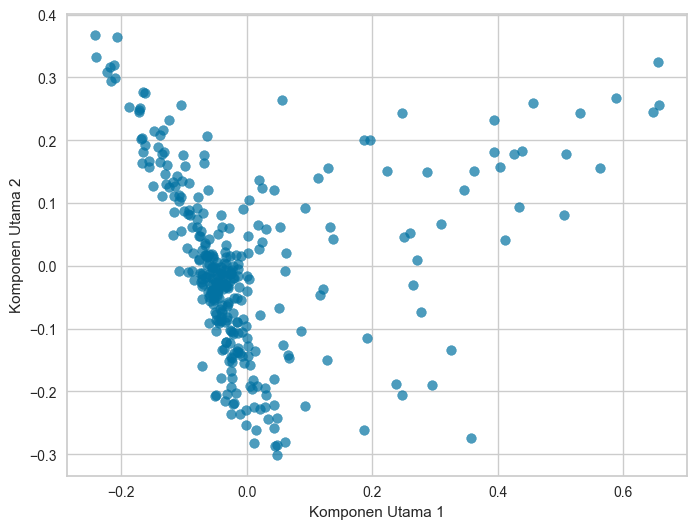
\includegraphics[width=0.7\linewidth]{img/4-221.png}
    \caption{Visualisasi hasil dari PCA}
    \label{fig:4-221}
\end{figure}

Setelah visualisasi PCA, langkah selanjutnya adalah melakukan K-Means \textit{clustering} untuk mengelompokkan abstrak menjadi beberapa klaster berdasarkan fitur TF-IDF yang telah direduksi menggunakan PCA. Pada implementasi KMeans, dibutuhkan satu parameter yaitu nilai dari K. Untuk menentukan nilai K atau jumlah \textit{num\_clusters} yang optimal, dilakukan pencarian dengan menampilkan \textit{Elbow Plot} menggunakan K-Means, dengan uji coba rentang klaster 1-10.

\begin{figure}[H]
    \centering
    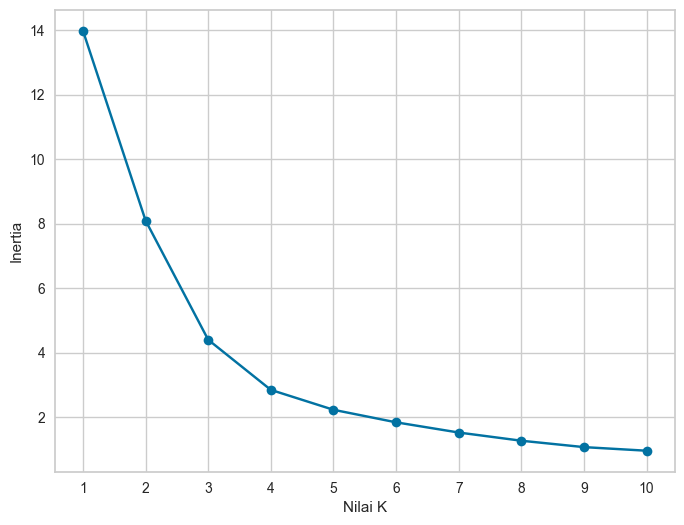
\includegraphics[width=0.725\linewidth]{img/4-21.png}
    \caption{\textit{Elbow Plot} untuk menentukan nilai klaster dengan K-Means}
    \label{fig:4-21}
\end{figure}

Dalam mempermudah penentuan nilai K yang optimum, dilakukan beberapa metrik evaluasi dengan \textit{Davies-Bouldin index} dan \textit{library ElbowVisualizer}, kedua metrik evaluasi tersebut digunakan untuk mengevaluasi nilai K yang optimal dalam algoritma K-Means. \textit{Davies-Bouldin index} mengukur kualitas pembagian klaster berdasarkan jarak antara klaster yang berdekatan dan dispersi internal setiap klaster \cite{sanghun2022}. Semakin rendah nilai \textit{Davies-Bouldin index}, semakin baik pembagian klaster dan semakin optimal nilai K yang digunakan. Selain itu, dengan \textit{library ElbowVisualizer} untuk membantu dan memperjelas dari visualisasi \textit{Elbow Plot}, pada saat titik di nilai \textit{inertia} mulai menurun secara lambat atau berhenti menurun drastis, itulah titik yang disarankan sebagai jumlah klaster yang optimal. Hasil dari kedua evaluasi tersebut menunjukkan nilai K=4 yang merupakan nilai K yang optimal, sehingga diterapkan fungsinya yakni \textit{KMeans(n\_clusters=4)}.

\begin{figure}[H]
    \centering
    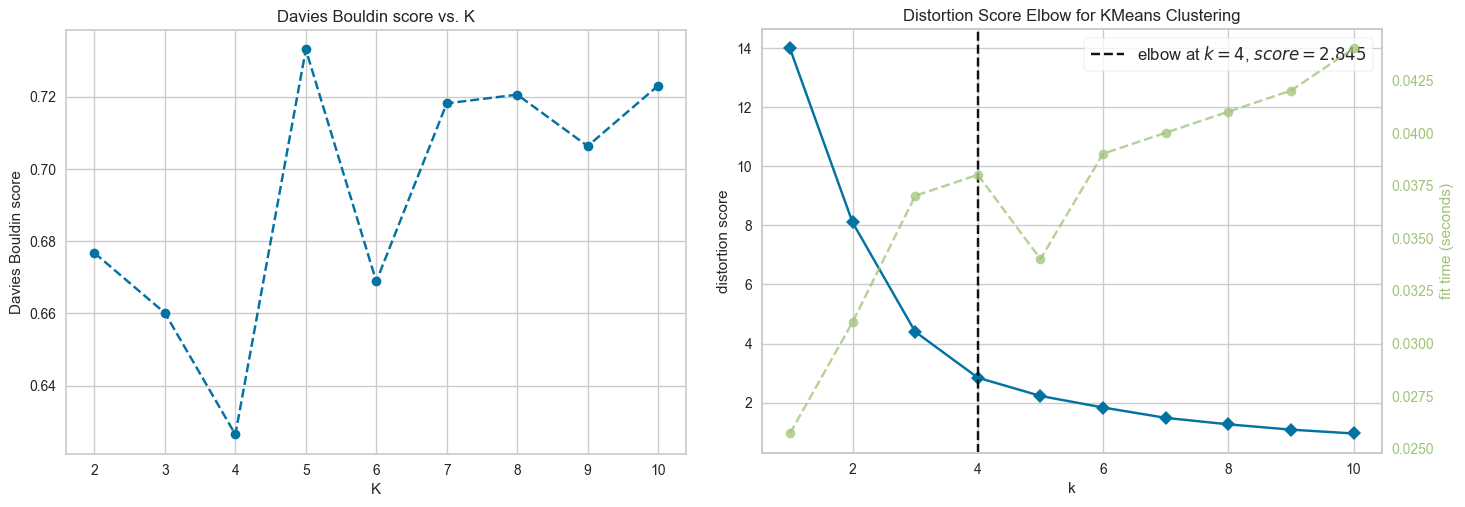
\includegraphics[width=0.9\linewidth]{img/4-21-3.png}
    \caption{Metrik Evaluasi nilai K dengan \textit{Davies-Bouldin index} dan \textit{library ElbowVisualizer}}
    \label{fig:4-21-3}
\end{figure}

Setelah melakukan K-Means \textit{clustering} dan menentukan jumlah klaster yang optimal berdasarkan \textit{elbow plot} dengan didukung validasi berupa evaluasi metrik, selanjutnya dapat diketahui dalam setiap klaster dengan menggunakan atribut dari objek K-Means untuk menyimpan label klaster pada setiap sampel data abstrak dan mengelompokkannya berdasarkan warna yang berbeda. 

Dalam konteks klasterisasi perwarnaan dengan K-Means, komponen utama 1 dan komponen utama 2 adalah dua dimensi baru yang dihasilkan dari PCA. Setiap baris data dalam dataset asli direpresentasikan oleh dua nilai pada komponen utama 1 dan komponen utama 2. Nilai-nilai ini menggambarkan lokasi relatif data dalam ruang dua dimensi yang telah direduksi. Pada saat PCA telah dilakukan, visualisasi data abstrak dalam ruang dua dimensi dengan \textit{scatter plot} menunjukkan bahwa setiap titik pada \textit{scatter plot} merepresentasikan satu abstrak, dan dapat dilihat berupa pola dan struktur data sebelum melakukan \textit{clustering}. 

\begin{figure}[H]
    \centering
    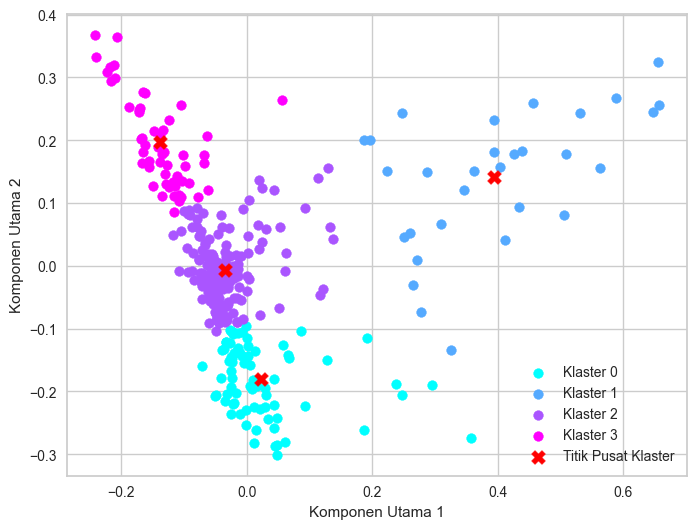
\includegraphics[width=0.7\linewidth]{img/4-222.png}
    \caption{Klasterisasi Pewarnaan dengan K-Means}
    \label{fig:4-222}
\end{figure}

% Selain itu, untuk mempermudah dalam melihat klaster mana yang lebih baik, dilakukanlah \textit{Silhouette plot} yang merupakan metode untuk mengukur seberapa baik setiap data abstrak dikelompokkan oleh K-Means. Plot ini menunjukkan nilai \textit{silhouette score} untuk setiap titik klaster pada data abstrak, nilai \textit{silhouette score} mengukur seberapa mirip data abstrak dengan kelompoknya sendiri dibandingkan dengan kelompok lain. \textit{Silhouette plot} juga membantu mengidentifikasi apakah ada kelompok yang tidak terdefinisi dengan baik atau apakah data abstrak tergolong dalam kelompok yang sesuai.

% \begin{figure}[H]
%     \centering
%     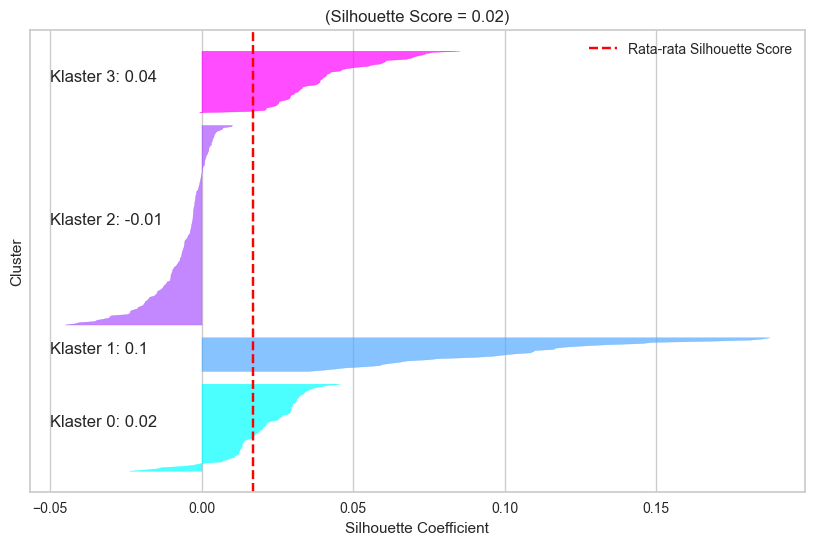
\includegraphics[width=0.7\linewidth]{img/4-23.png}
%     \caption{\textit{Silhouette Plot} untuk K-Means \textit{Clustering}}
%     \label{fig:4-23}
% \end{figure}

% Dari hasil tersebut, terdapat klaster yang memiliki warna yang menjulang jauh melebihi rata-rata dari \textit{Silhouette Score} yang telah didapatkan senilai 0.03 tersebut, yang menandakan bahwa klaster tersebut memiliki \textit{Silhouette Coefficient} yang tinggi dibandingkan dengan klaster lainnya. Klaster dengan \textit{Silhouette Coefficient} yang tinggi menunjukkan bahwa titik-titik data dalam klaster tersebut lebih dekat satu sama lain dan lebih terpisah dari titik-titik data di klaster lain. Hal ini, menunjukkan klaster tersebut memiliki titik-titik data yang sangat serupa dan kohesif. Dalam konteks analisis \textit{clustering}, hal ini dapat diartikan sebagai kelompok yang lebih homogen atau memiliki karakteristik yang sama. 

Pada keempat kluster yang berisi kelompok-kelompok abstrak tersebut, akan dipakai pada tahap selanjutnya, yaitu dilakukan penyeleksian dengan prinsip teori Luhn yang hasilnya nanti akan diterapkan suatu \textit{keyword extraction} untuk menentukan kata-kata kunci yang paling relevan dalam setiap klaster sebagai faktor dan sub-faktor GRK. 

\section{Hasil Pemilihan Kata Kunci berdasarkan Teori Luhn}
Pada tahapan memilih kata kunci, berdasarkan teori Luhn, data yang telah didapatkan dari hasil klasterisasi setiap kelompok, dilakukan suatu pemecahan kata-kata dasar pada masing-masing klaster dengan N-Grams = 1 (Unigram). 

\begin{table}[H]
\centering
\caption{Total jumlah kata setiap klaster}
\label{tab:jumlah_kata}
\resizebox{0.35\columnwidth}{!}{%
\begin{tabular}{l|c}
\hline
\textbf{Klaster} & \textbf{Total Jumlah Kata} \\
\hline
\textit{Cluster 0} & \textit{13198 Kata} \\
\textit{Cluster 1} & \textit{8137 Kata} \\
\textit{Cluster 2} & \textit{2473 Kata} \\
\textit{Cluster 3} & \textit{6476 Kata} \\
\hline
\end{tabular}%
}
\end{table}


Setelah dilakukan proses pemecahan menjadi kata-kata dasar pada setiap klaster, didapatkan jumlah kata yang didapatkan sebagaimana yang telah ditunjukkan pada Tabel \ref{tab:jumlah_kata}. Kemudian untuk melihat suatu frekuensi dari masing-masing kata dasar, terdapat visualisasi dengan \textit{Word cloud} untuk menunjukkan representasi visual dari data teks yang menggambarkan frekuensi kata-kata dalam teks tersebut \cite{hicke_word_2022}. Dalam \textit{word cloud}, kata-kata yang muncul lebih sering akan ditampilkan dengan ukuran yang lebih besar, sedangkan kata-kata yang muncul lebih jarang akan ditampilkan dengan ukuran yang lebih kecil. 

\begin{figure}[H]
    \centering
    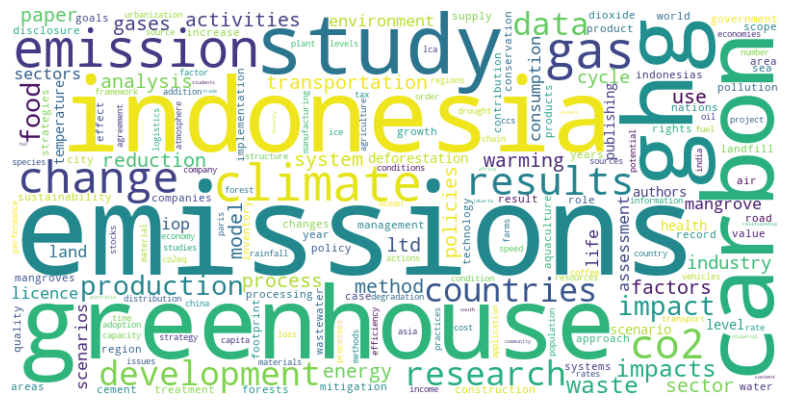
\includegraphics[width=0.6\linewidth]{img/4-31-1.png}
    \caption{Representasi visual frekuensi data dengan \textit{word cloud} pada \textit{Cluster 0}}
    \label{fig:4-31-1}
\end{figure}
\begin{figure}[H]
    \centering
    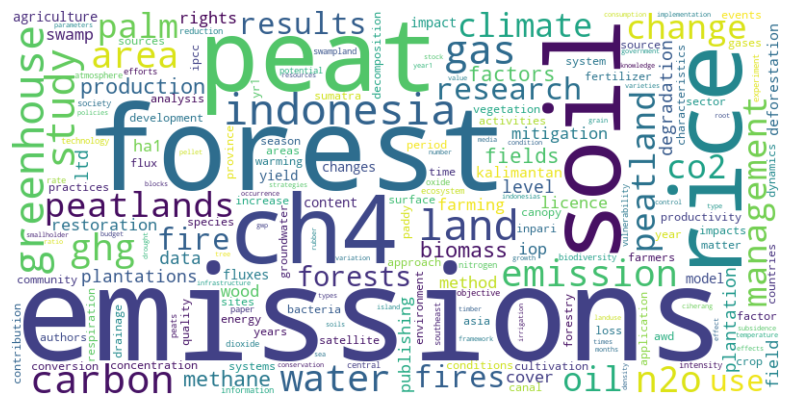
\includegraphics[width=0.6\linewidth]{img/4-31-2.png}
    \caption{Representasi visual frekuensi data dengan \textit{word cloud} pada \textit{Cluster 1}}
    \label{fig:4-31-2}
\end{figure}
\begin{figure}[H]
    \centering
    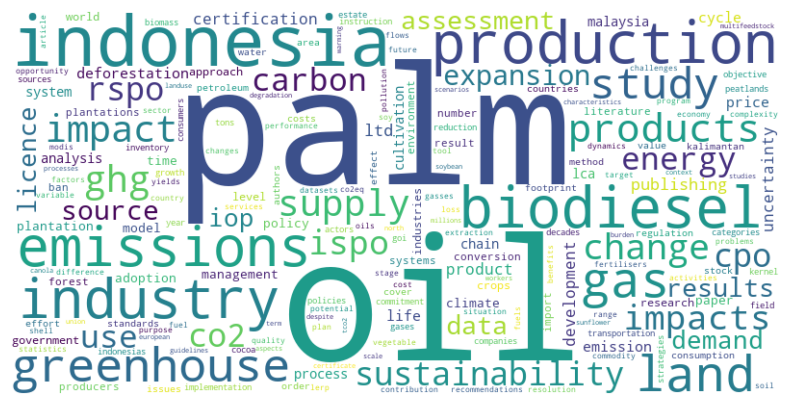
\includegraphics[width=0.6\linewidth]{img/4-31-3.png}
    \caption{Representasi visual frekuensi data dengan \textit{word cloud} pada \textit{Cluster 2}}
    \label{fig:4-31-3}
\end{figure}
\begin{figure}[H]
    \centering
    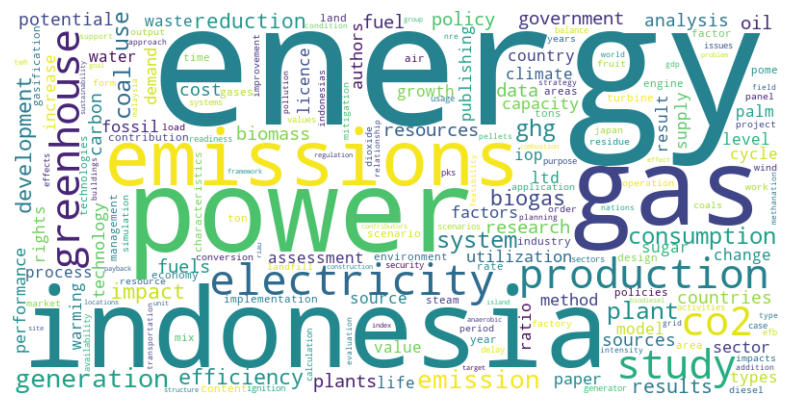
\includegraphics[width=0.6\linewidth]{img/4-31-4.png}
    \caption{Representasi visual frekuensi data dengan \textit{word cloud} pada \textit{Cluster 3}}
    \label{fig:4-31-4}
\end{figure}

Pada keempat representasi visual menggunakan \textit{word cloud} sebelumnya, bisa dilihat bahwa masing-masing setiap klaster memiliki unsur kata dengan jumlah frekuensi yang cukup sedikit berbeda. Terlihat pula kata-kata dasar apa yang memiliki ukuran paling besar dan yang kecil. Namun, pada tahapan seleksi teori Luhn ini bukanlah memilih kata-kata yang memiliki frekuensi terbesar, melainkan semua data dengan jumlah frekuensi kata pada setiap klaster yang akan dipakai pada tahapan teori Luhn. Adapun bagian-bagian kata yang memiliki frekuensi terbesar dan frekuensi terkecil akan dibuang, karena berdasarkan teori Luhn, interval data pada rentang tersebut merupakan istilah-istilah yang kurang baik dalam memilih kata kunci yang relevan secara optimal.

Berikut adalah langkah-langkah dalam pemilihan kata-kata dari hasil \textit{clustering} dan penerapan teori Luhn, serta \textit{labelling} faktor dan subfaktor pada setiap klasternya sebagai berikut:

\begin{enumerate}
    \item Pemisahan Kalimat Abstrak menjadi Kata-Kata Dasar: Pada setiap klaster, semua kalimat abstrak akan dipecah menjadi kata-kata dasar. Hal tersebut membantu mengidentifikasi kata-kata kunci yang paling mewakili konten dari setiap klaster.
    \item Perhitungan Frekuensi Kemunculan Kata: Frekuensi kemunculan setiap kata dalam klaster dihitung. Dengan informasi ini, didapatkan gambaran tentang kata-kata yang paling sering muncul dalam konteks klaster tertentu.
    \item Penerapan Teori Luhn: Prinsip teori Luhn digunakan untuk memilih kata-kata yang memiliki frekuensi kemunculan di dalam interval yang ditentukan. Interval ini mengarahkan untuk menghilangkan beberapa kata yang mungkin terlalu umum atau terlalu jarang muncul. Tujuannya adalah mendapatkan kata-kata kunci yang lebih relevan.
    \item Penentuan Batas: Berdasarkan teori Luhn, batas interval ditentukan. Batas ini mencakup lower cut (batas bawah) dan upper cut (batas atas). Kata-kata kunci yang masuk dalam interval ini memiliki potensi sebagai representasi yang tepat dari faktor penyebab GRK.
    \item Seleksi Kata-Kata Kunci: Kata-kata kunci yang memiliki frekuensi kemunculan di dalam interval batas akan dipilih. Ini menghasilkan kumpulan kata-kata kunci yang akan mewakili konten klaster tertentu.
    \item Analisis Kualitatif: Setelah kata-kata kunci dipilih, dilakukan analisis kualitatif lebih lanjut secara manual. Setiap kata kunci akan ditafsirkan dalam konteks faktor penyebab Gas Rumah Kaca (GRK). Hal ini melibatkan pemahaman mendalam tentang makna kata-kata, serta bagaimana kata-kata tersebut terkait dengan aspek GRK.
    \item \textit{Labelling} Faktor dan Subfaktor: Setelah analisis kualitatif, kata-kata kunci tersebut dapat digunakan sebagai label untuk mengidentifikasi faktor dan subfaktor GRK dalam setiap klaster. Label ini memberikan representasi komprehensif tentang apa yang mendasari peningkatan GRK.
\end{enumerate}

Setelah melakukan langkah-langkah tersebut pada setiap klaster, maka didapatkanlah faktor dan sub-faktor GRK yang relevan dengan menggunakan kata-kata kunci yang telah dipilih. Proses ini juga merupakan interpretasi akhir mengenai aspek atau faktor penyebab GRK dalam masing-masing konteks klaster.

\section{Hasil Interpretasi Kata Kunci Berdasarkan Teknik \textit{Clustering} dan Seleksi Teori Luhn}

\begin{table}[H]
\centering
\caption{Hasil Kata Kunci yang Terpilih berdasarkan teknik Clustering dan implementasi teori Luhn}
\label{tab:factors}
\resizebox{0.95\columnwidth}{!}{%
\begin{tabular}{|l|l|p{0.95\textwidth}|}
\hline
\multicolumn{3}{|c|}{\textbf{Faktor dan 10 Subfaktor Aspek GRK di Indonesia berdasarkan Kata Kunci yang Dihasilkan}} \\ \hline
\textbf{Klaster} & \textbf{Faktor} & \textbf{Subfaktor} \\ \hline
\textit{Cluster 0} & \textit{Deforestation} & \textit{emissions peat, deforestation degradation, mangrove deforestation, mangrove carbon, deforestation mangroves, emissions peatlands, vegetation indices, land fires, emissions peat, forestry land} \\ \hline
\textit{Cluster 1} & \textit{Biodiesel} & \textit{biodiesel production, biomass indonesia, indonesias palm, palm peatlands, biodiesel palm, palm oil, impacts biodiesel, footprint biodiesel, palm expansion, biofuel role} \\ \hline
\textit{Cluster 2} & \textit{co2 / Carbon} & \textit{buildings co2emissions, co2 cement, co2resistant cementing, coal power, waste composition, co2 atmosphere, dependence fuels, contributors carbon, waste business, pollutants countries} \\ \hline
\textit{Cluster 3} & \textit{Electricity} & \textit{electricity consumption, policies energy, buildings energy, boiler efficiency, electricity supply, energy policy, generator efficiency, indonesian electricity, energy sources, capacity biogas} \\ \hline
\end{tabular}%
}
\end{table}



% \begin{table}[H]
% \caption{Hasil Kata Kunci yang Terpilih Berdasarkan Teknik \textit{Clustering} dan Implementasi Teori Luhn}
% \label{tab:kata_kunci_terpilih}
% \resizebox{\columnwidth}{!}{%
% \begin{tabular}{@{}|l|p{0.8\textwidth}|@{}}
% \midrule
% \multicolumn{3}{c}{\textbf{Faktor dan 10 Subfaktor Aspek GRK di Indonesia berdasarkan Kata Kunci yang Dihasilkan }}                                        \\ \midrule
% \textit{\textbf{Cluster 0}} & \textit{Deforestation} & \textit{emissions peat, eforestation degradation, mangrove deforestation, mangrove carbon, deforestation mangroves, emissions peatlands, vegetation indices, land fires, emissions peat, forestry land}                                                        \\ \midrule
% \textit{\textbf{Cluster 1}}          & \textit{emissions, forest, soil, peat, rice, ch4, indonesia, greenhouse, land, gas, study, carbon, water, ghg, n2o, emission, area, peatlands, management, palm}                                                    \\ \midrule
% \textit{\textbf{Cluster 2}}          & \textit{oil, palm, emissions, indonesia, production, gas, greenhouse, biodiesel, industry, ghg, study, soil, land, forest, peat, plantations, n2o, carbon, co2, impact}                                                                            \\ \midrule
% \textit{\textbf{Cluster 3}}          & \textit{energy, power, indonesia, gas, emissions, electricity, production, greenhouse, co2, study, generation, emission, plant, consumption, ghg, coal, system, use, biogas, efficiency}                                                               \\  \bottomrule
% \end{tabular}%
% }
% \end{table}

% \begin{itemize}
    % \item [a.] \textbf{\textit{Cluster 0}}: \textit{emissions, indonesia, greenhouse, carbon, ghg, study, emission, gas, climate, change, co2, results, development, research, countries, data, production, impact, food, impacts}
    % \item [b.] \textbf{\textit{Cluster 1}}: \textit{emissions, forest, soil, peat, rice, ch4, indonesia, greenhouse, land, gas, study, carbon, water, ghg, n2o, emission, area, peatlands, management, palm}
    % \item [c.] \textbf{\textit{Cluster 2}}: \textit{oil, palm, indonesia, production, biodiesel, emissions, industry, gas, land, greenhouse, study, products, impact, supply, ghg, change, impacts, ispo, cpo, rspo}
    % \item [d.] \textbf{\textit{Cluster 3}}: \textit{energy, power, indonesia, gas, emissions, electricity, production, greenhouse, co2, study, generation, emission, plant, consumption, ghg, coal, system, use, biogas, efficiency}
% \end{itemize}

Setelah dilakukan suatu pemilihan kata-kata kunci dari gabungan hasil proses teknik \textit{clustering} dan prinsip teori Luhn tersebut, berdasarkan sumber dari data studi literatur, aspek dan faktor penyebab dari GRK yang ada di Indonesia, maka dari hasil tersebut bisa dijadikan sebagai landasan secara efektif untuk melihat kondisi saat ini dengan memanfaatkan studi literatur 5 tahun terakhir yang membahas terkait subjek atau urgensi perihal GRK di Indonesia. 

Contohnya seperti \textit{emissions peat, deforestation degradation, mangrove deforestation} yang merupakan subfaktor dari faktor \textit{deforestation} dan faktor klaster lainnya yang memiliki keterkaitan antara sesama kata-kata kunci yang bisa digabungkan menjadi frasa berupa subfaktor seperti contoh tersebut. Oleh karena itu, dari hasil penelitian ini, dari kata-kata kunci yang didapatkan, dapat diketahui faktor dan subfaktor atau bahkan aspek hal lainnya yang bisa menjadi perhatian bahwa dengan memanfaatkan teknologi saat ini seperti \textit{Artificial Intellegence} dan juga analisis data yang didukung juga berdasarkan teori, dapat membantu dalam analisis tersebut, terutama dalam mengetahui hal-hal yang berhubungan dengan aspek yang dicari.